\documentclass[border=8pt]{standalone}
\usepackage[T1]{fontenc}\usepackage[utf8]{inputenc}
\usepackage{helvet}\renewcommand{\familydefault}{\sfdefault}
\usepackage{tikz,xcolor}
\usetikzlibrary{arrows.meta,positioning,shapes.geometric,shapes.multipart,calc,fit,backgrounds,decorations.markings}
\definecolor{ink}{HTML}{1E1B16}\definecolor{paper}{HTML}{FBF8F2}\definecolor{clay}{HTML}{B5482A}\definecolor{soft}{HTML}{F1E9DA}\definecolor{pine}{HTML}{24402F}
\tikzset{
  every node/.style={font=\small,text=ink},
  >=Stealth, line/.style={draw=ink,line width=0.8pt},
  cls/.style={rectangle split,rectangle split parts=3,draw=ink,line width=0.8pt,fill=soft,align=left,inner xsep=6pt,inner ysep=4pt,
              rectangle split part align={center,left,left},minimum width=3.0cm},
  cls2/.style={rectangle split,rectangle split parts=2,draw=ink,line width=0.8pt,fill=soft,align=left,inner xsep=6pt,inner ysep=4pt,
              rectangle split part align={center,left},minimum width=3.0cm},
  box/.style={rectangle,draw=ink,line width=0.8pt,fill=soft,align=center,inner sep=5pt,minimum height=0.8cm},
  state/.style={rectangle,rounded corners=8pt,draw=ink,line width=0.8pt,fill=soft,align=center,inner sep=6pt,minimum width=2.2cm,minimum height=0.9cm},
  act/.style={rectangle,rounded corners=10pt,draw=ink,line width=0.8pt,fill=soft,align=center,inner sep=5pt,minimum width=2.4cm,minimum height=0.8cm},
  dec/.style={diamond,draw=ink,line width=0.8pt,fill=soft,inner sep=1pt,minimum width=0.9cm,minimum height=0.9cm},
  uc/.style={ellipse,draw=ink,line width=0.8pt,fill=soft,align=center,inner sep=3pt,minimum width=3.2cm,minimum height=1.0cm},
  note/.style={rectangle,draw=ink,line width=0.6pt,fill=yellow!12,align=left,inner sep=4pt,font=\footnotesize},
  lab/.style={font=\footnotesize,fill=paper,inner sep=1.5pt},
  err/.style={},
}
\newcommand{\actor}[3]{% x,y,label
  \draw[line width=0.8pt] (#1,#2+0.55) circle (0.17);
  \draw[line width=0.8pt] (#1,#2+0.38)--(#1,#2-0.15) (#1-0.3,#2+0.22)--(#1+0.3,#2+0.22) (#1,#2-0.15)--(#1-0.25,#2-0.6) (#1,#2-0.15)--(#1+0.25,#2-0.6);
  \node[font=\small] at (#1,#2-0.9) {#3};}
\begin{document}
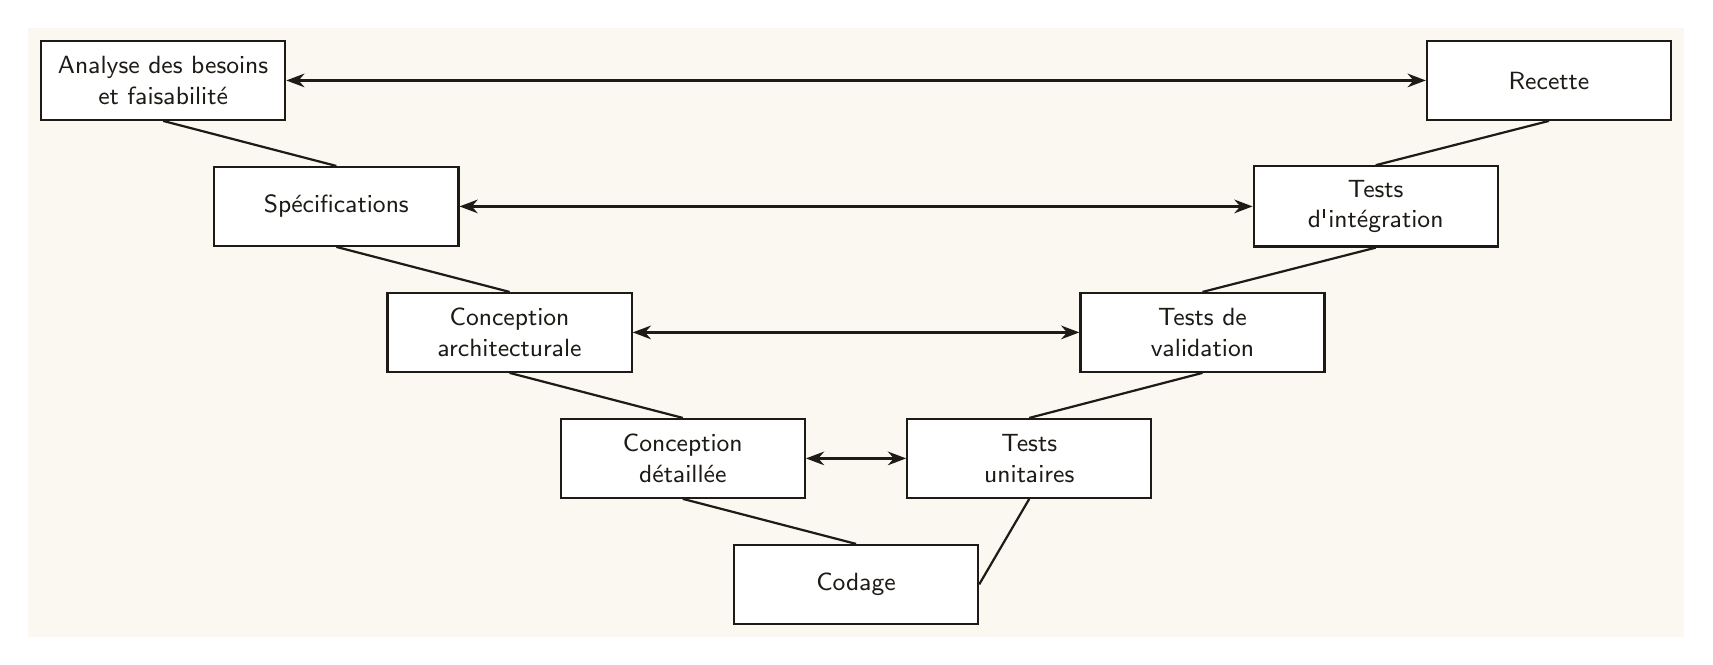
\begin{tikzpicture}[background rectangle/.style={fill=paper},show background rectangle]
\node[box,minimum width=3.1cm,minimum height=1.0cm,fill=white] (l0) at (0.1999999999999993,6.4) {Analyse des besoins\\et faisabilit\'e};
\node[box,minimum width=3.1cm,minimum height=1.0cm,fill=white] (l1) at (2.4000000000000004,4.8) {Sp\'ecifications};
\node[box,minimum width=3.1cm,minimum height=1.0cm,fill=white] (l2) at (4.6,3.2) {Conception\\architecturale};
\node[box,minimum width=3.1cm,minimum height=1.0cm,fill=white] (l3) at (6.8,1.6) {Conception\\d\'etaill\'ee};
\node[box,minimum width=3.1cm,minimum height=1.0cm,fill=white] (l4) at (9.0,0.0) {Codage};
\node[box,minimum width=3.1cm,minimum height=1.0cm,fill=white] (r0) at (17.8,6.4) {Recette};
\node[box,minimum width=3.1cm,minimum height=1.0cm,fill=white] (r1) at (15.6,4.8) {Tests\\d\textquotesingle int\'egration};
\node[box,minimum width=3.1cm,minimum height=1.0cm,fill=white] (r2) at (13.4,3.2) {Tests de\\validation};
\node[box,minimum width=3.1cm,minimum height=1.0cm,fill=white] (r3) at (11.2,1.6) {Tests\\unitaires};
\draw[line] (l0.south)--(l1.north);
\draw[line] (l1.south)--(l2.north);
\draw[line] (l2.south)--(l3.north);
\draw[line] (l3.south)--(l4.north);
\draw[line] (l4.east)--(r3.south);
\draw[line] (r3.north)--(r2.south);
\draw[line] (r2.north)--(r1.south);
\draw[line] (r1.north)--(r0.south);
\draw[line,<->] (l0.east)--(r0.west);
\draw[line,<->] (l1.east)--(r1.west);
\draw[line,<->] (l2.east)--(r2.west);
\draw[line,<->] (l3.east)--(r3.west);
\end{tikzpicture}
\end{document}
